\documentclass[../notes.tex]{subfiles}

\pagestyle{main}
\renewcommand{\chaptermark}[1]{\markboth{\chaptername\ \thechapter\ (#1)}{}}
\setcounter{chapter}{3}

\begin{document}




\chapter{Central Conservative Forces}
\section{Conservation Laws, Radial Energy Equation, Orbits}
\begin{itemize}
    \item \marginnote{10/16:}Review.
    \begin{itemize}
        \item The Lagrangian for a free particle.
        \item We have that space is isotropic and homogeneous, and time is homogeneous.
        \item $L(v^2)$ or $L(v)$ implies that the equations of motion are invariant under the velocity boost.
        \item Recall that $v=\sqrt{v^2}=\sqrt{v_x^2+v_y^2+v_z^2}$.
        \item From here, we get to $L=\frac{1}{2}mv^2$
    \end{itemize}
    \item What we've said on 3D central conservative forces thus far.
    \begin{itemize}
        \item Consider a particle in 3D at position $\vec{r}$ being acted on by external forces $\vec{F}(\vec{r})$.
        \item In spherical coordinates, we have
        \begin{align*}
            x &= r\sin\theta\cos\phi&
            y &= r\sin\theta\sin\phi&
            z &= r\cos\theta
        \end{align*}
        \begin{itemize}
            \item $\theta$ is the \textbf{polar} angle.
            \item $\phi$ is the \textbf{azimuthal} angle.
        \end{itemize}
        \item Special case: \emph{Central} force.
        \begin{itemize}
            \item \emph{Central} force: Acts in a direction parallel to $\vec{r}$.
            \item Thus, if $\vec{F}$ is central, then $\vec{G}=\vec{r}\times\vec{F}=0$. It follows that $\vec{J}=\vec{r}\times\vec{p}$ is conserved.
        \end{itemize}
        \item Special case: \emph{Conservative} force.
        \begin{itemize}
            \item Condition: $\vec{\nabla}\times\vec{F}=0$.
            \item In this case, there exists a scalar function $V$ such that $\vec{F}=-\vec{\nabla}V$.
            \item Equivalently, in spherical coordinates,
            \begin{align*}
                F_r &= -\pdv{V}{r}&
                F_\theta &= -\frac{1}{r}\pdv{V}{\theta}&
                F_\phi &= -\frac{1}{r\sin\theta}\pdv{V}{\phi}
            \end{align*}
            \item Thus, since $F_\theta=F_\phi=0$, it follows that $V=V(r)$ is not dependent on $\theta$ or $\phi$. Mathematically,
            \begin{equation*}
                \vec{F} = -\pdv{F}{r}\hat{r}
            \end{equation*}
        \end{itemize}
    \end{itemize}
    \item Recall: Uniform circular motion.
    \begin{itemize}
        \item In plane polar coordinates, we have
        \begin{equation*}
            \vec{F} = m\ddot{\vec{r}} = m[(\ddot{r}-r\dot{\theta}^2)\hat{r}+(r\ddot{\theta}+2\dot{r}\dot{\theta})\hat{\theta}]
        \end{equation*}
        \item In uniform circular motion, $\dot{\theta}=\omega$ and $r=R$, so we get
        \begin{equation*}
            \vec{F} = mR\omega^2\hat{r}
            = \frac{mv^2}{R}\hat{r}
        \end{equation*}
        \begin{itemize}
            \item Note that to get from the second expression above to the third one, we substitute the definition of angular velocity: $\omega=v/R$.
        \end{itemize}
    \end{itemize}
    \item We are now ready to treat the case of the \emph{central conservative} force.
    \begin{itemize}
        \item Herein, we get a lot of conservation laws!
        \begin{enumerate}
            \item Energy is conserved:
            \begin{equation*}
                \frac{1}{2}m\dot{\vec{r}}{\,}^2+V(r) = E = \text{constant}
            \end{equation*}
            \begin{itemize}
                \item Note that this is a scalar equation.
            \end{itemize}
            \item Angular momentum is conserved:
            \begin{equation*}
                m\vec{r}\times\dot{\vec{r}} = \vec{J} = \text{constant}
            \end{equation*}
            \begin{itemize}
                \item Note that this is a set of 3 vector equations.
            \end{itemize}
        \end{enumerate}
        \item Letting $r,\theta$ be our plane polar coordinates, we can rewrite equation (1) above as follows.
        \begin{equation*}
            \frac{1}{2}m(\dot{r}^2+r^2\dot{\theta}^2)+V(r) = E
        \end{equation*}
        \item Similarly, we can rewrite equation (2) above as follows.
        \begin{align*}
            \vec{J} &= mr\hat{r}\times(\underbrace{\dot{r}}_{v_r}\hat{r}+\underbrace{r\dot{\theta}}_{v_\theta}\hat{\theta})\\
            J &= mr^2\dot{\theta}
        \end{align*}
        \begin{itemize}
            \item Note that $J$ is a scalar here.
        \end{itemize}
        \item Since $\dot{\theta}$ is a function of $r$, we get orbits??
        \item In particular, if we plug $\dot{\theta}=J/mr^2$ into the original conservation of energy equation, we get the \textbf{radial energy equation}.
    \end{itemize}
    \item \textbf{Radial energy equation}: The equation defined as follows. \emph{Given by}
    \begin{equation*}
        \frac{1}{2}m\dot{r}^2+\frac{J^2}{2mr^2}+V(r) = E
    \end{equation*}
    \begin{itemize}
        \item Note that this looks a lot like the original energy conservation law once we define the \textbf{effective potential energy}.
    \end{itemize}
    \item \textbf{Effective potential energy}: The following expression, which treats a radial particle as if it were a one-dimensional particle, i.e., in a rotating reference frame. \emph{Denoted by} $\bm{U(r)}$. \emph{Given by}
    \begin{equation*}
        U(r) = \frac{J^2}{2mr^2}+V(r)
    \end{equation*}
    \item Example: $V(r)=kr^2/2$.
    \begin{itemize}
        \item Then $U(r)=J^2/2mr^2+kr^2/2$. We get a shape that is a blend of a parabola but that goes up super steeply as we approach the axis.
        \item We have a PE function that looks like a parabola, but gets steeper close to the origin; this gives us two turn about points.
    \end{itemize}
    \item Most important example: The inverse square law.
    \begin{figure}[h!]
        \centering
        \begin{subfigure}[b]{0.3\linewidth}
            \centering
            \begin{tikzpicture}
                \small
                \draw
                    (0,-1) -- (0,3) node[above]{$U(r)$}
                    (0,0) -- (3,0) node[right]{$r$}
                ;
    
                \footnotesize
                \draw (0.924,0.1) -- ++(0,-0.2) node[below]{$r_1$};
                \draw [densely dashed] (0,2) node[left]{$E$} -- ++(3,0);
    
                \draw [blx,thick] plot[domain=0.69:3,smooth] (\x,{0.6/(\x)^2+1.2/\x});
            \end{tikzpicture}
            \caption{$k>0$.}
            \label{fig:invSqPota}
        \end{subfigure}
        \begin{subfigure}[b]{0.3\linewidth}
            \centering
            \begin{tikzpicture}
                \small
                \draw
                    (0,-1) -- (0,3) node[above]{$U(r)$}
                    (0,0) -- (3,0) node[right]{$r$}
                ;
    
                \footnotesize
                \draw (0.5,0.1) -- ++(0,-0.2) node[below,xshift=-1pt]{$\frac{\ell}{2}$};
                \draw (1,0.1) -- ++(0,-0.2) node[below]{$\ell$};
                \draw (0.1,-0.6) -- ++(-0.2,0) node[left]{$-\frac{|k|}{2\ell}$};
    
                \draw [blx,thick] plot[domain=0.29:3,samples=100,smooth] (\x,{0.6/(\x)^2-1.2/\x});
            \end{tikzpicture}
            \caption{$k<0$.}
            \label{fig:invSqPotb}
        \end{subfigure}
        \caption{Potentials under the inverse square law.}
        \label{fig:invSqPot}
    \end{figure}
    \begin{itemize}
        \item Attractive and repulsive case.
        \item Occurs when $\vec{F}=k\hat{r}/r^2$.
        \item $k>0$ is repulsive (think like charges).
        \item $k<0$ is attractive (think gravity or opposite charges).
        \item Repulsive case ($k>0$):
        \begin{itemize}
            \item We have
            \begin{equation*}
                U(r) = \frac{J^2}{2mr^2}+\frac{k}{r}
            \end{equation*}
            \item Thus, we get a point of closest approach as dictated by the energy $E$, but that's it.
        \end{itemize}
        \item Attractive case:
        \begin{itemize}
            \item We have
            \begin{equation*}
                U(r) = \frac{J^2}{2mr^2}+\frac{k}{r}
            \end{equation*}
            once again.
            \item If we define the \textbf{length scale}, then we obtain
            \begin{equation*}
                U(r) = |k|\left( \frac{\ell}{2r^2}-\frac{1}{r} \right)
            \end{equation*}
            \item It follows that, as in Figure \ref{fig:invSqPotb}, the effective potential crosses $y=0$ at $\ell/2$ and has minimum at $y=-|k|/2\ell$.
            \item Additionally, there are four possible types of trajectories depending on the value of $E$.
            \begin{enumerate}
                \item ($E=U_\text{min}=-|k|/2\ell$): $\vec{r}=0$, and we get uniform circular motion with $r=\vec{l}$. The kinetic energy is
                \begin{equation*}
                    \frac{1}{2}mv^2 = T
                    = E-V
                    = -\frac{|k|}{2\ell}-\frac{k}{\ell}
                    = \frac{|k|}{2\ell}
                \end{equation*}
                so that the speed is
                \begin{equation*}
                    v = \sqrt{\frac{|k|}{m\ell}}
                \end{equation*}
                \item ($-|k|/2\ell<E<0$): Bounded orbit between $r_1<r<r_2$. The shape is an \emph{ellipse}, as we will later prove.
                \item ($E=0$): The orbit is a parabola: It comes in, slingshots around, and just escapes back to $\infty$.
                \item ($E>0$): The orbit is a hyperbola.
            \end{enumerate}
        \end{itemize}
    \end{itemize}
    \item \textbf{Length scale}: The distance from the origin at which the particle orbits stably. \emph{Denoted by} $\bm{\ell}$. \emph{Given by}
    \begin{equation*}
        \ell = \frac{J^2}{m|k|}
    \end{equation*}
    \item We find the orbits by eliminating time from the radial energy equation.
    \begin{itemize}
        \item Recall that
        \begin{equation*}
            \frac{1}{2}m\dot{r}^2+\frac{J^2}{2mr^2}+V(r) = E
        \end{equation*}
        \item Now substitute in $u=1/r$ and its consequence $\dv*{u}{\theta}=(-1/r^2)\dv*{r}{\theta}$. Note, of course, that we are just encoding all of the information in $r$ in this "$u$."
        \item It follows that
        \begin{equation*}
            \dot{r} = \dv{r}{\theta}\dot{\theta}
            = -r^2\dot{\theta}\dv{u}{\theta}
            = -\frac{J}{m}\dv{u}{\theta}
        \end{equation*}
        \item Returning the substitution into the radial energy equation, we obtain
        \begin{equation*}
            \frac{J^2}{2m}\left( \dv{u}{\theta} \right)^2+\frac{J^2}{2m}u^2+V(u) = E
        \end{equation*}
        \item Evidently, this equation relates $u$ to $\theta$ for a given potential energy function $V$!
        \item We can use this equation to solve for the $V(u)$ that gives us an orbit $u(\theta)$, and (even easier) we can solve for the orbit given $V(u)$. Depending on how complicated this is, we may not be able to solve the ODE. But we \emph{can} solve it in several cool cases.
    \end{itemize}
    \item We'll start next time with orbits of the inverse square law.
\end{itemize}



\section{Office Hours (Jerison)}
\begin{itemize}
    \item Is the $L$ $\to$ $mv^2/2$ derivation in any textbook?
    \begin{itemize}
        \item No, but she will post it.
    \end{itemize}
    \item What do the Lagrangian and action \emph{mean}?
    \begin{itemize}
        \item The Lagrangian is $T-V$ to some extent because that's what gives us Newton's laws when we extremize it. It doensn't have to be this way, but this is the math that makes everything work out.
        \item $T$ is a function of the velocities and $V$ of the positions (for conservative forces).
        \item A \emph{necessary} condition: If $L$ satisfies Lagrange's EOMs, then $S$ is a stationary point.
        \item The action really doesn't mean anything for the system; it happens that this is another way to formulate mechanics, but the principle of least action is just as empirical as Newton's laws.
        \item She didn't have any good examples for $S$ in the $(x,v,t)$ space, but I'll try to come up with one. Maybe on uniform constant-velocity 1D motion.
    \end{itemize}
    \item Constraint equations in Problem 1?
    \begin{itemize}
        \item Just rewrite constraints in the form $f(q_i,t)=0$ and take derivatives.
    \end{itemize}
    \item An example of using Lagrange undetermined multipliers: Let's tackle the parabolic wire again.
    \begin{itemize}
        \item Let our bead be confined to the wire which has shape $y=\alpha x^2$. Let gravity act in the $-\jhat$ direction. Let the particle have mass $m$.
        \item As per usual, write the Lagrangian as $L=T-V$. Instead of immediately using the constraint equations to get rid of a certain variable, we'll keep it and modify EOMs.
        \item Take $T=m(\dot{x}^2+\dot{y}^2)/2$ and $V=mgy$.
        \item Since we didn't substitute out variables using the constraint, we have to add an additional generalized force to the EOM:
        \begin{equation*}
            \dv{t}(\pdv{L}{\dot{q}_i})-\pdv{L}{q_i}+\sum_j\lambda_j(t)\pdv{f_j}{q_i} = 0
        \end{equation*}
        \item Constraint: $f_1(x,y)=y-\alpha x^2=0$.
        \item Since we have 2 variables and 1 constraint, substituting everything in, we get 3 equations:
        \begin{align*}
            \dv{t}(m\dot{x})+\lambda_1(t)(-2\alpha x) &= 0&
            \dv{t}(m\dot{y})-mg+\lambda_1(t) &= 0&
            y-\alpha x^2 &= 0
        \end{align*}
        \begin{itemize}
            \item We use the same $\lambda$ both times because each $\lambda$ corresponds to the single constraint, $f_1$.
        \end{itemize}
        \item Simplifying, we obtain
        \begin{align*}
            m\ddot{x}-2\alpha x\lambda(t) &= 0&
            m\ddot{y}-mg+\lambda(t) &= 0&
            y-\alpha x^2 &= 0
        \end{align*}
        \item To solve for $\lambda$ in terms of $y$, rewrite equation 2:
        \begin{equation*}
            \lambda(t) = mg-m\ddot{y}
        \end{equation*}
        \item Since $\ddot{y}=2\alpha\dot{x}^2+2\alpha x\ddot{x}$ and the force of constraint is $\lambda_1(t)\pdv*{f_1}{q_i}$, we obtain
        \begin{equation*}
            \lambda(t) = mg-m(2\alpha\dot{x}^2+2\alpha x\ddot{x})
        \end{equation*}
        \item This allows us to plug back into equation 1 to get
        \begin{equation*}
            m\ddot{x}-2\alpha x(mg-m(2\alpha\dot{x}^2+2\alpha x\ddot{x})) = 0
        \end{equation*}
        \item And we get back to the generic nonlinear ODE. So even if we slice the parabolic wire problem this way, we still can't solve for the motion analytically.
        \item Notice how we used all three equations in the system to get to the final EOM above!
    \end{itemize}
    \item When would the method of Lagrange multipliers be a faster method than direct substitution?
    \begin{itemize}
        \item There are some types of constraints that are easier to do like this, but we aren't ready for any of those examples yet.
        \item Right now, the main utility of this perspective is allowing for the generalized force of constraint to pop out so that we get this extra piece of information. It's not yet computationally simpler.
    \end{itemize}
    \item Why does problem 2 exist?
    \begin{itemize}
        \item It's one of the ways of deriving the plane polar coordinates we've used so often.
        \item Question: What is the correct expression for acceleration in plane polar coordinates. We need
        \begin{equation*}
            \ddot{\vec{r}} = \pdv[2]{t}(r\hat{r})
        \end{equation*}
        \item So 2 is partially Newtonian and partially Lagrange multiplier. The Newtonian way is complicated; the other way is simpler.
    \end{itemize}
    \item How do we find $\omega$ in Problem 3?
    \begin{itemize}
        \item There is a correct period that is dictated by the requirement that if you look out at it, it looks like it is not moving.
        \item For Question 3, we have full license to define our own variables and then look up their values online.
        \item For instance,
        \begin{equation*}
            \vec{F} = -\frac{GMm}{r^2}\hat{r}
        \end{equation*}
    \end{itemize}
    \item Problem 5:
    \begin{itemize}
        \item We won't need to look up any info about Kepler's laws, but we can if we want/need for context.
    \end{itemize}
    \item Problem 4:
    \begin{itemize}
        \item Question 4.9, not 3.9.
        \item We can write an effective potential energy function; we know that circular motion occurs at the minimum.
        \item There are several ways to solve this. An easier way actually might be with $mv^2/r$.
    \end{itemize}
    \item The $V(r)=kr^2/2$ example from class?
    \begin{itemize}
        \item There's a derivation of this in Section 4.1 of \textcite{bib:KibbleBerkshire}. We can find the orbits using the equation relating potentials to orbits. The isotropic harmonic oscillator gives elliptical orbits.
        \item Ellipses look like oscillations if we only look at them radially.
        \item In this case, it's \emph{not} spiralling in any funny way. There are some that do, but not this one.
    \end{itemize}
    \item What does the effective potential energy give us?
    \begin{itemize}
        \item It means that radially, the particle behaves as a particle in the 1D potential $U(r)$.
    \end{itemize}
\end{itemize}



\section{Inverse Square Law, Scattering}
\begin{itemize}
    \item \marginnote{10/18:}Logistical announcements.
    \begin{itemize}
        \item We're in week 4 now!
        \item Next week: Chapter 5. This will conclude Midterm 1 material.
        \item We'll cover new material on 10/30 and 11/1, but they won't be on the midterm.
        \item There will be an outline of all Midterm 1 content.
        \item Logistical survey on Canvas very soon.
    \end{itemize}
    \item Today.
    \begin{itemize}
        \item Counting degrees of freedom.
        \item Orbits of the inverse square law.
    \end{itemize}
    \item Recap.
    \begin{itemize}
        \item A central conservative force can be written as follows.
        \begin{equation*}
            \vec{F}(\vec{r}) = -\dv{V}{r}\hat{r}
        \end{equation*}
        \item This is a special, constrained scenario due to conservation laws.
    \end{itemize}
    \item A new perspective on this scenario: Define it in terms of \textbf{degrees of freedom} and, especially, what happens to them when we apply various conservation laws.
    \item \textbf{Degree of freedom}: A piece of information that you need to specify the future trajectory of a particle. \emph{Also known as} \textbf{DOF}, \textbf{independent coordinate}.
    \item Example.
    \begin{itemize}
        \item 1 particle in 3D has 6 DOFs: $(x,y,z,\dot{x},\dot{y},\dot{z})$.
        \item The corresponding initial conditions $(x_0,y_0,z_0,\dot{x}_0,\dot{y}_0,\dot{z}_0)$ suffice to specify the complete future trajectory of the particle.
    \end{itemize}
    \item Continuing with this example, what if we start adding in constraints?
    \begin{itemize}
        \item If this particle in 3D is under a \emph{central} force, then the \emph{direction} of $\vec{J}$ is conserved.
        \begin{itemize}
            \item This corresponds to a loss of 2 DOFs.
            \item In particular, if the direction of $\vec{J}$ is constant, then the particle's motion is constrained to the plane to which $\vec{J}$ is normal.
            \item Thus, position and velocity normal to this plane are both zero, and we've lost 2 DOFs.
            \item Note that this loss is easy to see in a coordinate system that takes the plane to which $\vec{J}$ is normal to be the $xy$-plane, or something. Then $z=\dot{z}=0$ for all time. However, in an alternate coordinate system, the DOFs are still lost; it's just expressed by the fact that changing one of the six coordinates \emph{necessarily} changes at least one of the others.
        \end{itemize}
        \item Additionally, if this particle in 3D is under a central force, then $|\vec{J}|$ and $E$ are also fixed.
        \begin{itemize}
            \item This removes two more DOFs, one per constraint.
            \item For starters,
            \begin{equation*}
                |\vec{J}| = mr^2\dot{\theta}
            \end{equation*}
            relates $\dot{\theta}$ to $r$.
            \item Additionally,
            \begin{equation*}
                \frac{1}{2}m(\dot{r}^2+r^2\dot{\theta}^2)+V(r) = E
            \end{equation*}
            relates $\dot{r}$ to $r$.
        \end{itemize}
        \item At this point, the shape of the orbit is determined; the only things we can still pick are the particle's starting location $\vec{r}_0$ and the orientation of the plane of the orbit with respect to the coordinate system.
        \begin{itemize}
            \item The choices of these two things essentially allow us to specify the coordinate system in which our "affine" orbit takes place.
        \end{itemize}
    \end{itemize}
    \item We now dive into orbits for the inverse square law, the most important case of a central force.
    \begin{itemize}
        \item Example inverse square forces.
        \begin{itemize}
            \item In gravity, $k=-GMm$.
            \item In Coulomb, $k=qq'/4\pi\varepsilon_0$.
        \end{itemize}
        \item Reminders.
        \begin{itemize}
            \item For $F=-k/r^2$, $V(r)=k/r$.
            \item Defining $u=1/r$ gives $V(u)=ku$.
            \item $k<0$ is attractive and $k>0$ is repulsive.
            \item Rewriting the conservation laws into more friendly forms yields the radial energy equation (with effective potential energy) and an \textbf{orbit equation}.
        \end{itemize}
        \item We now analyze the orbit equation relevant to the inverse square law, which is reiterated below for clarity. Guiding question: What orbits are possible?
        \begin{equation*}
            \frac{J^2}{2m}\left( \dv{u}{\theta} \right)^2+\frac{J^2}{2m}u^2+ku = E
        \end{equation*}
        \begin{itemize}
            \item Define the length scale as before. Substituting it into the above equation and multiplying through by $2/|k|$, we obtain
            \begin{equation*}
                \ell\left( \dv{u}{\theta} \right)^2+\ell u^2\pm 2u = \frac{2E}{|k|}
            \end{equation*}
            \item Rearrange and simplify:
            \begin{align*}
                \ell\left( \dv{u}{\theta} \right)^2+\ell u^2\pm 2u &= \frac{2E}{|k|}\\
                \ell^2\left( \dv{u}{\theta} \right)^2+\ell^2u^2\pm 2u\ell+1 &= \frac{2E\ell}{|k|}+1\\
                \ell^2\left( \dv{u}{\theta} \right)^2+(\ell u\pm 1)^2 &= \frac{2E\ell}{|k|}+1
            \end{align*}
            \item Now, let
            \begin{align*}
                z &= \ell u\pm 1&
                e^2 &= \frac{2E\ell}{|k|}+1
            \end{align*}
            so that
            \begin{equation*}
                \dv{z}{\theta} = \dv{z}{u}\dv{u}{\theta}
                = \ell\dv{u}{\theta}
            \end{equation*}
            \item Then
            \begin{equation*}
                \left( \dv{z}{\theta} \right)^2+z^2 = e^2
            \end{equation*}
            \item The solution to this differential equation is
            \begin{equation*}
                z = e\cos(\theta-\theta_0)
            \end{equation*}
            where $\theta_0$ is a constant of integration.
            \item Setting the above equal to the original definition of $z$ --- $\ell u\pm 1$ --- we can find the final trajectories
            \begin{align*}
                e\cos(\theta-\theta_0) &= \ell u\pm 1\\
                e\cos(\theta-\theta_0)\mp 1 &= \frac{\ell}{r}\\
                r(e\cos(\theta-\theta_0)\mp 1) &= \ell
            \end{align*}
        \end{itemize}
        \item These equations are called \textbf{conic sections}.
        \begin{itemize}
            \item If $k>0$, we get repulsive:
            \begin{equation*}
                r(e\cos(\theta-\theta_0)-1) = \ell
            \end{equation*}
            \item If $k<0$, we get attractive:
            \begin{equation*}
                r(e\cos(\theta-\theta_0)+1) = \ell
            \end{equation*}
        \end{itemize}
        \item Note that we call the constant $e$ the \textbf{eccentricity} and $\theta_0$ the \textbf{orientation}.
    \end{itemize}
    \item \textbf{Eccentricity}: A dimensionless quantity that discriminates amongst various types of orbits. \emph{Denoted by} $\bm{e}$.
    \begin{itemize}
        \item $e=0 \Longrightarrow \text{circle}$.
        \item $e<1 \Longrightarrow \text{ellipse}$.
        \item $e>1 \Longrightarrow \text{hyperbola}$.
        \item $e=1 \Longrightarrow \text{parabola}$.
    \end{itemize}
    \item We typically let the origin of our coordinate system lie at one focus or the orbit.
    \item Relating energy $E$ and eccentricity $e$.
    \begin{itemize}
        \item Recall that
        \begin{equation*}
            e^2-1 = \frac{2E\ell}{|k|}
        \end{equation*}
        \item Thus\dots
        \begin{itemize}
            \item $E>0$ implies $e^2>1$, i.e., a hyperbolic orbit.
            \item $E<0$ implies $e<1$, i.e., an elliptical orbit.
            \item $E=0$ implies $e=1$, i.e., a parabolic orbit.
        \end{itemize}
        \item Lastly, the minimum energy that such a system can have occurs when $e=0$. In this case, the energy is
        \begin{equation*}
            E_\text{min} = -\frac{|k|}{2\ell}
        \end{equation*}
        \begin{itemize}
            \item Note that this can only occur under an attractive force; otherwise, looking back at the trajectory, we'd have $r=-\ell$.
            \item This should also make intuitive sense, as to have uniform circular motion, we do need an \emph{attractive} central force.
        \end{itemize}
        \item In the case of a repulsive force, we necessarily have $E>0$ and a hyperbola. $k$ is independent here.
    \end{itemize}
    \item Now, let's further analyze the case of elliptic orbits.
    \begin{figure}[h!]
        \centering
        \begin{tikzpicture}
            \footnotesize
            \draw (-3.5,0) -- (1.5,0);
            \draw (0,-1.5) -- (0,1.5);
            \draw (-1,0.1) -- ++(0,-0.2) node[below]{$-ae$};
    
            \draw [rex,thick,dashed] (-1,0) -- node[right,black]{$b$} (-1,1);
            \draw [rex,thick,dashed] (-1,0) -- node[above,black]{$a$} (-3,0);
            \node [below right,yshift=-1mm] {0};
            \draw (-0.1,{3^0.5/2}) -- ++(0.2,0) node[right,yshift=2pt]{$\ell$};
    
            \draw [rex,thick] (-1,0) ellipse (2cm and 1cm);
        \end{tikzpicture}
        \caption{Elliptic orbits.}
        \label{fig:orbitsElliptic}
    \end{figure}
    \begin{itemize}
        \item $E<0\Longrightarrow 0\leq e\leq 1$, and $k<0$ by necessity.
        \item In Cartesian coordinates, the equation for an ellipse is
        \begin{equation*}
            \frac{(x+ae)^2}{a^2}+\frac{y^1}{b^2} = 1
        \end{equation*}
        where
        \begin{align*}
            a &= \frac{\ell}{1-e^2}&
            b &= \frac{\ell}{\sqrt{1-e^2}}
        \end{align*}
        \item $a$ is the \textbf{semimajor axis length}; $b$ is the \textbf{semiminor axis length}; $\ell$ is known as the \textbf{semilatus rectum} in this context; the center of attraction lies at one of the ellipse's foci, which lies at the origin; and the center of the ellipse is at $(-ae,0)$ relative to this coordinate system.
        \item Cartesian and polar form of the ellipse? See Appendix B in \textcite{bib:KibbleBerkshire}.
    \end{itemize}
    \item Elliptic orbit constant relations.
    \begin{itemize}
        \item The scale of the orbit is fixed by $E$ since
        \begin{equation*}
            a = \frac{\ell}{1-e^2} = \frac{|k|}{2|E|}
        \end{equation*}
        \item $\ell$ is determined by $J$ since
        \begin{equation*}
            b^2 = a\ell = \frac{J^2}{2m|E|}
        \end{equation*}
    \end{itemize}
    \item We now investigate determine period $\tau$ of the orbit.
    \begin{itemize}
        \item Since we are investigating a central force, our system satisfies Kepler's second law:
        \begin{equation*}
            \dv{A}{t} = \frac{J}{2m}
        \end{equation*}
        \item Equivalently,
        \begin{equation*}
            \dv{t}{A} = \frac{2m}{J}
        \end{equation*}
        \begin{itemize}
            \item Physically, this means that the time $t$ it takes for the particle to sweep out an area $A$ is $t=\dv*{t}{A}\cdot A=2mA/J$.
        \end{itemize}
        \item In particular, this means that the period (the time it takes the particle to sweep out a full ellipse of area $A=\pi ab$) is
        \begin{equation*}
            \tau = \pi ab\cdot\frac{2m}{J}
        \end{equation*}
    \end{itemize}
    \item We now look at a consequence of this definition of the period.
    \item \textbf{Kepler's third law}: The square of the period is proportional to the cube of the semimajor axis. \emph{Given by}
    \begin{equation*}
        \tau^2 \propto a^3
    \end{equation*}
    \item Derivation.
    \begin{itemize}
        \item Essentially, since $b^2=a\ell$ by the above and $\ell=J^2/m|k|$ by definition, we have that
        \begin{align*}
            \tau &= \pi ab\cdot\frac{2m}{J}\\
            \frac{\tau}{2\pi} &= \frac{mab}{J}\\
            \left( \frac{\tau}{2\pi} \right)^2 &= \frac{m^2a^2b^2}{J^2}\\
            &= \frac{m^2a^2(a\ell)}{m|k|\ell}\\
            &= \frac{m}{|k|}a^3\\
            \tau^2 &\propto a^3
        \end{align*}
        \item Note that in the particular case of gravity, where $|k|=GMm$, we have
        \begin{align*}
            \left( \frac{\tau}{2\pi} \right)^2 &= \frac{a^3}{GM}
        \end{align*}
    \end{itemize}
    \item This concludes our investigation of elliptic orbits.
    \item We now investigate hyperbolic orbits.
    \begin{figure}[h!]
        \centering
        \begin{tikzpicture}
            \footnotesize
            \draw (-1.5,0) -- (3.5,0);
            \draw (0,-2.5) -- (0,2.5);
    
            % \draw (1,0.1) -- ++(0,-0.2) node[below]{$ae$};
            \draw [help lines]
                (1,0.1) -- (1,-1.7)
                (1.5,0.1) -- (1.5,-1.7)
            ;
            \draw [<->,shorten <=1pt,shorten >=1pt] (0,-1.6) -- node[below]{$ae$} ++(1,0);
            \draw [<->,shorten <=1pt,shorten >=1pt] (1,-1.6) -- node[below]{$a$} ++(0.5,0);
            \draw [<->,shorten <=1pt,shorten >=1pt] (0,0) -- node[below left=-2pt]{$b$} ++(0.5,-0.5);
            \node [left] at (0,{3^0.5/4}) {$\ell$};
    
            \coordinate (A) at (3.5,0);
            \coordinate (B) at (1,0);
            \coordinate (C) at (3,2);
            % \pic [draw,angle radius=4.5mm,angle eccentricity=0.8,pic text={\tiny$\theta_1$}] {angle=A--B--C};
            \pic [draw,<->,shorten <=1pt,shorten >=1pt,angle radius=7mm,angle eccentricity=1.3,pic text={$\theta_1$}] {angle=A--B--C};
            \coordinate (D) at (-1,2);
            % \pic [draw,angle radius=4.5mm,angle eccentricity=0.7,pic text={\tiny$\Theta$}] {angle=C--B--D};
            \pic [draw,<->,shorten <=1pt,shorten >=1pt,angle radius=7mm,angle eccentricity=1.3,pic text={$\Theta$}] {angle=C--B--D};
    
            \draw [white,line width=4pt] (1.3,-0.3) -- ++(0.4,-0.4);
            \draw [rex,semithick,dashed]
                (-1,-2) -- (3,2)
                (-1,2) -- (3,-2)
            ;
    
            \draw [white,line width=3pt] plot[domain=0.2:0.5,variable=\y,smooth,/pgf/fpu,/pgf/fpu/output format=fixed] ({1+(0.5^2*(1+\y*\y/0.5^2))^0.5},\y);
            \draw [white,line width=3pt] plot[domain=-0.5:-0.2,variable=\y,smooth,/pgf/fpu,/pgf/fpu/output format=fixed] ({1-(0.5^2*(1+\y*\y/0.5^2))^0.5},\y);
    
            \draw [rex,thick,decoration={markings,mark=at position 0.2 with \arrow{>},mark=at position 0.8 with \arrow{>}},postaction={decorate}] plot[domain=-2:2,variable=\y,smooth,/pgf/fpu,/pgf/fpu/output format=fixed] ({1+(0.5^2*(1+\y*\y/0.5^2))^0.5},\y);
            \draw [rex,thick,decoration={markings,mark=at position 0.2 with \arrow{>},mark=at position 0.8 with \arrow{>}},postaction={decorate}] plot[domain=-2:2,variable=\y,smooth,/pgf/fpu,/pgf/fpu/output format=fixed] ({1-(0.5^2*(1+\y*\y/0.5^2))^0.5},\y);
        \end{tikzpicture}
        \caption{Hyperbolic orbits.}
        \label{fig:orbitsHyperbolic}
    \end{figure}
    \begin{itemize}
        \item $E>0\Longrightarrow e>1$, but $k$ can be positive or negative.
        \begin{itemize}
            \item If $k>0$, then per the above, $r(e\cos\theta-1)=\ell$ and the particle follows the trajectory described by the right branch of the hyperbola in Figure \ref{fig:orbitsHyperbolic}, coming near it and being pushed away.
            \item If $k<0$, then per the above, $r(e\cos\theta+1)=\ell$ and the particle follows the trajectory described by the left branch of the hyperbola in Figure \ref{fig:orbitsHyperbolic}, coming near it and being slingshot around.
        \end{itemize}
        \item In Cartesian coordinates, the equation for a hyperbola is
        \begin{equation*}
            \frac{(x-ae)^2}{a^2}-\frac{y^2}{b^2} = 1
        \end{equation*}
        where
        \begin{align*}
            a &= \frac{\ell}{e^2-1} = \frac{|k|}{2E}&
            b^2 &= a\ell = \frac{J^2}{2mE}
        \end{align*}
        \item $b$ is known as the \textbf{impact parameter} in this context (because it tells you how close the particle would get to the center of attraction/repulsion if it continued in a straight line along the directrix) and $\Theta$ is the \textbf{scattering angle}.
    \end{itemize}
    \item We now investigate the scattering angle more wholistically.
    \begin{itemize}
        \item To calculate $\theta_1$, notice that in the repulsive case, the particle has polar coordinate $\theta_1$ when $r=\infty$. But according to the polar equations, $r\to\infty$ implies that $e\cos\theta-1\to 0$ if the product is to stay equal to $\ell$. Thus, when $r=\infty$, we have
        \begin{align*}
            e\cos\theta_1-1 &= 0\\
            \theta_1 &= \cos^{-1}\left( \tfrac{1}{e} \right)\\
            &= \cos^{-1}\left( \tfrac{1}{e} \right)
        \end{align*}
        \item The hyperbola is symmetric in the attractive case, so the scattering angle $\Theta$ is given by
        \begin{equation*}
            \Theta = \pi-2\theta_1 = \pi-2\cos^{-1}\left( \tfrac{1}{e} \right)
        \end{equation*}
    \end{itemize}
    \item The scattering angle can be used to calculate the impact parameter as follows.
    \begin{itemize}
        \item It follows by rearranging the above equation that
        \begin{equation*}
            e = \sec\left[ \tfrac{1}{2}(\pi-\Theta) \right]
        \end{equation*}
        \item Thus, the facts that $a=\ell/(e^2-1)$ and $b^2=a\ell$ along with the trig identity $\sec^2[(\pi-x)/2]-1=\cot^2(x/2)$ imply that
        \begin{align*}
            \frac{a\ell}{e^2-1} &= a^2\\
            \frac{b^2}{e^2-1} &= a^2\\
            b^2 &= a^2(e^2-1)\\
            &= a^2(\sec^2\left[ \tfrac{1}{2}(\pi-\Theta) \right]-1)\\
            &= a^2\cot^2\left( \tfrac{1}{2}\Theta \right)
        \end{align*}
        \item We'll finish this derivation next time.
    \end{itemize}
\end{itemize}



\section{Scattering}
\begin{itemize}
    \item \marginnote{10/20:}Today.
    \begin{itemize}
        \item Solid angle + differential cross-section.
        \item Hard sphere scattering.
        \item Rutherford scattering.
    \end{itemize}
    \item Recap.
    \begin{itemize}
        \item A central conservative force obeys
        \begin{equation*}
            \vec{F}(\vec{r}) = -\hat{r}\dv{V}{r}
        \end{equation*}
        \begin{itemize}
            \item $\vec{J}$ and $E$ are both conserved.
            \item 2 degrees of freedom: Starting location and orientation with respect to the coordinate system.
        \end{itemize}
        \item A particle under a central conservative force satisfies the orbit equation
        \begin{equation*}
            \frac{J^2}{2m}\left( \dv{u}{\theta} \right)^2+\frac{J^2}{2m}u^2+V(u) = E
        \end{equation*}
        where $u=1/r$.
        \begin{itemize}
            \item This equation relates the potential energy (or \textbf{force law}) to the \emph{shape} of the orbit.
        \end{itemize}
        \item Under an inverse square law force, $V(u)=ku$. In this case, the orbits are given by
        \begin{align*}
            r[e\cos(\theta-\theta_0)-1] &= \ell\tag{$k>0$}\\
            r[e\cos(\theta-\theta_0)+1] &= \ell\tag{$k<0$}
        \end{align*}
        where
        \begin{align*}
            \ell &= \frac{J^2}{m|k|}&
            e^2-1 &= \frac{2E\ell}{|k|}
        \end{align*}
    \end{itemize}
    \item Continuing with last time's derivation: Calculating the impact parameter $b$ as a function of the scattering $\Theta$.
    \begin{itemize}
        \item Last time, we learned that
        \begin{equation*}
            b(\Theta) = a\cot\left( \tfrac{1}{2}\Theta \right)
        \end{equation*}
        \item Let $v$ be the particle's velocity at $r=\infty$. Then $E=mv^2/2$. Substituting this into the previous result $a=|k|/2E$ yields
        \begin{equation*}
            a = \frac{|k|}{mv^2}
        \end{equation*}
        \item Thus,
        \begin{equation*}
            b(\Theta) = \frac{|k|}{mv^2}\cot\left( \tfrac{1}{2}\Theta \right)
        \end{equation*}
    \end{itemize}
    \item We are now ready to discuss particle scattering.
    \item Consider a single particle with initial velocity $v$ traveling horizontally within a certain reference frame so that it approaches the scattering center at the origin with impact parameter $b$.
    \begin{figure}[h!]
        \centering
        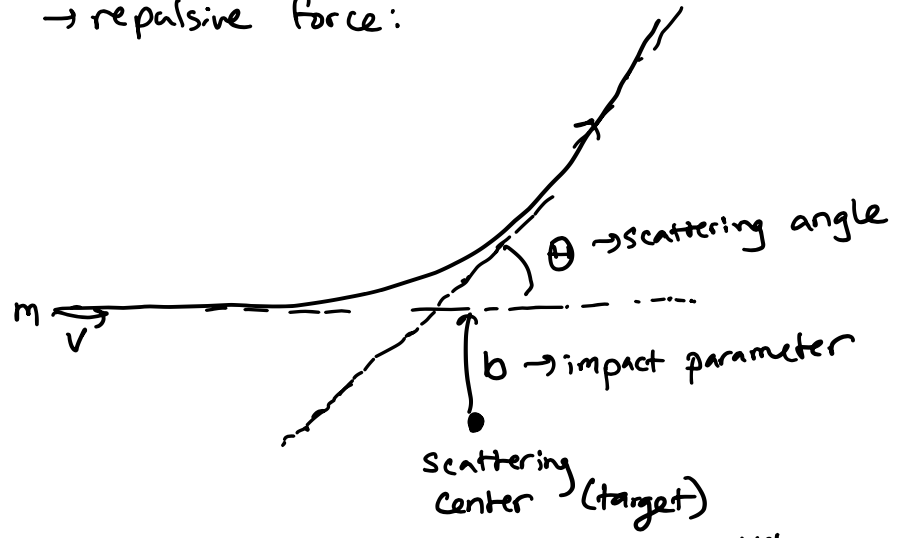
\includegraphics[width=0.4\linewidth]{../ExtFiles/scatteringSP.png}
        \caption{Scattering of a single particle.}
        \label{fig:scatteringSP}
    \end{figure}
    \begin{itemize}
        \item Approaching at the distance $b$, we know via the above that the particle (if under an inverse square law force) leaves with scattering angle $\Theta$ where $b=|k|/mv^2\cdot\cot(\Theta/2)$.
    \end{itemize}
    \item Now consider a range of particles landing on a detector subtending angles $\dd\phi,\dd\theta$ at scattering angle $\theta$.
    \begin{figure}[h!]
        \centering
        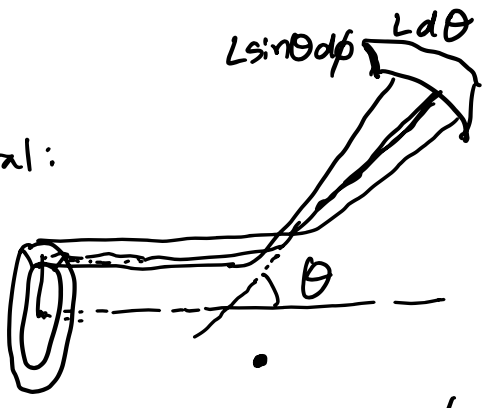
\includegraphics[width=0.3\linewidth]{../ExtFiles/scatteringMP.png}
        \caption{Scattering of multiple particles.}
        \label{fig:scatteringMP}
    \end{figure}
    \begin{itemize}
        \item These particles would come from an impact parameter range $(b,b+\dd{b})$.
        \item If the particle has interacted with the scattering center and is now a distance $L$ from it (where we assume $L\gg b$), then the area of the detector is given by
        \begin{equation*}
            \dd{A} = L^2\sin\theta\dd\theta\dd\phi
        \end{equation*}
        \item Per the above image, we define the area that produces particles that scatter at angle $\theta$ into solid angle $\sin\theta\dd\theta\dd\phi$ as $\dd\sigma=b\dd\phi\cdot\dd{b}$.
        \item Let $I$ be the intensity of the particle beam in units of particles/area/time.
        \item Then the \textbf{differential scattering cross-section} is given by
        \begin{equation*}
            \dv{\sigma}{\Omega} = \frac{Ib\dd{b}\dd\phi}{-I\sin\theta\dd\theta\dd\phi}
            = \frac{b}{\sin\theta}\left| \dv{b}{\theta} \right|
        \end{equation*}
        \begin{itemize}
            \item Note that we have the negative sign in the denominator because $\dv*{b}{\theta}$ is typically negative.
            \item Alternatively, we are taking the ratio of a \emph{positive} flux of incoming particles to a \emph{negative} flux of outgoing particles.
        \end{itemize}
        \item Denote the number of particles hitting the detector (per unit time) by $\dd{w}$. Then
        \begin{equation*}
            \dd{w} = I\dd\sigma = I\dv{\sigma}{\Omega}\frac{\dd{A}}{L^2}
        \end{equation*}
    \end{itemize}
    \item \textbf{Solid angle}: The sphere-area element analogous to $\dd\theta$ on a circle. \emph{Denoted by} $\bm{\textbf{d}\Omega}$. \emph{Given by}
    \begin{equation*}
        \dd\Omega = \sin\theta\dd\theta\dd\phi
    \end{equation*}
    \begin{itemize}
        \item Intuition: Using the solid angle, we can calculate the surface area of the unit sphere as follows.
        \begin{equation*}
            \iint_\text{sphere}\dd\Omega = \int_0^{2\pi}\int_0^\pi\sin\theta\dd\theta\dd\phi = 4\pi
        \end{equation*}
    \end{itemize}
    \item \textbf{Differential scattering cross-section}: The rate of scattering particles per unit solid angle at angle $\theta$. \emph{Also known as} \textbf{differential cross-section}. \emph{Denoted by} $\bm{\textbf{d}\sigma/\textbf{d}\Omega}$.
    \begin{itemize}
        \item Generally, the differential scattering cross section is a function of the scattering angle $\theta$.
    \end{itemize}
    \item We now investigate two types of scattering.
    \item Example 1: Hard sphere scattering.
    \begin{figure}[h!]
        \centering
        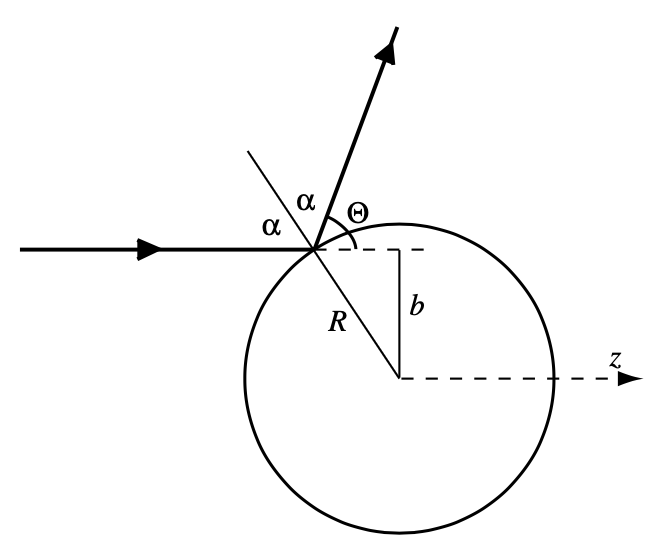
\includegraphics[width=0.35\linewidth]{../ExtFiles/scatteringHS.png}
        \caption{Hard sphere scattering.}
        \label{fig:scatteringHS}
    \end{figure}
    \begin{itemize}
        \item From Figure \ref{fig:scatteringHS}, we can read off that
        \begin{equation*}
            \alpha = \frac{\pi-\theta}{2}
        \end{equation*}
        \item It follows considering the triangle within the sphere that the central angle $\beta$ is given by
        \begin{equation*}
            \beta = \frac{\pi}{2}-\alpha
            = \frac{\pi}{2}-\frac{\pi-\theta}{2}
            = \frac{\theta}{2}
        \end{equation*}
        \item Thus, the impact parameter and scattering angle are related via simple trigonometry:
        \begin{equation*}
            \cos\frac{\theta}{2} = \frac{b}{R}
        \end{equation*}
        \item It follows that
        \begin{equation*}
            \dv{b}{\theta} = -\frac{1}{2}R\sin\frac{\theta}{2}
        \end{equation*}
        \item Hence,
        \begin{equation*}
            \dv{\sigma}{\Omega} = \frac{b}{\sin\theta}\left| \dv{b}{\theta} \right|
            = \frac{R\cos(\frac{\theta}{2})}{2\sin(\frac{\theta}{2})\cos(\frac{\theta}{2})}\cdot\frac{1}{2}R\sin\left( \frac{\theta}{2} \right)
            = \frac{R^2}{4}
        \end{equation*}
        \begin{itemize}
            \item Note that the differential scattering cross-section is isotropic (i.e., does not depend on the scatterng angle) in this case!
        \end{itemize}
        \item Note: Intuitively, the total area $\sigma$ that scatters particles should be equal to the cross-sectional area of the target. We can check that it is here as follows.
        \begin{equation*}
            \sigma = \iint_\text{sphere}\dv{\sigma}{\Omega}\dd\Omega
            = \int_0^{2\pi}\int_0^\pi\frac{R^2}{4}\sin\theta\dd\theta\dd\phi
            = \pi R^2
        \end{equation*}
    \end{itemize}
    \item Example 2: Rutherford scattering.
    \begin{itemize}
        \item This is analogous to the case of alpha particles and gold nuclei, which repel under an inverse square law force!
        \item As before, we may invoke the following general result for scattering (regardless of force):
        \begin{equation*}
            \dv{\sigma}{\Omega} = \frac{b}{\sin\theta}\left| \dv{b}{\theta} \right|
        \end{equation*}
        \item Let's assemble the components of the above.
        \begin{itemize}
            \item First off, $b=a\cot(\theta/2)$ since we're working with an inverse square law force.
            \item Next, $\sin\theta=2\sin(\theta/2)\cos(\theta/2)$.
            \item Finally, we may use the first result to determine that $\dv*{b}{\theta}=-a/2\sin^2(\theta/2)$.
        \end{itemize}
        \item Putting everything back together, we obtain
        \begin{equation*}
            \dv{\sigma}{\Omega} = a\cdot\frac{\cos(\theta/2)}{\sin(\theta/2)}\cdot\frac{1}{2\sin(\theta/2)\cos(\theta/2)}\cdot\frac{a}{2\sin^2(\theta/2)}
            = \frac{a^2}{4\sin^4(\theta/2)}
        \end{equation*}
        \item Moreover, note that $a=|k|/mv^2=qq'/4\pi\varepsilon_0mv^2$ because the Coulomb force in question is between an alpha particle of charge $q$ and gold nuclei of charge $q'$. Thus, alternatively,
        \begin{equation*}
            \dv{\sigma}{\Omega} = \frac{a^2{q'}^2}{64\pi^2\varepsilon_0^2m^2v^4\sin^4(\theta/2)}
        \end{equation*}
        \begin{itemize}
            \item Thus, the number of particles hitting a certain detector scales with $q^2{q'}^2=Z^2{Z'}^2$ for nuclei, is strongly dependent on $v$, and is anisotropic with $\dv*{\sigma}{\Omega}$ at its minimum with respect to $\theta$ when $\theta=\pi$.
        \end{itemize}
    \end{itemize}
    \item Mean free path and scattering in materials.
    \item Consider a particle moving through a material containing $n$ atoms per unit volume (this quantity is a \textbf{number density}).
    \begin{itemize}
        \item Let $\sigma$ denote the total scattering cross-section per atom.
        \item Thus, in a path of length $x$, we would expect the particle to collide with $n\sigma x$ atoms ($n$ is a number density and $\sigma x$ is a volume).
        \item It follows that the \textbf{mean free path} is the value $x=\lambda$ such that $n\sigma\lambda=1$.
    \end{itemize}
    \item \textbf{Mean free path}: The typical distance the particle travels between collisions. \emph{Denoted by} $\bm{\lambda}$. \emph{Given by}
    \begin{equation*}
        \lambda = \frac{1}{n\sigma}
    \end{equation*}
    \item We can now answer questions such as, "how far do particles penetrate into a material?"
    \begin{itemize}
        \item Consider a beam of particles with an incident flux of $f$ particles/unit area/unit time.
        \item Let $f(x)$ denote the flux of particles at penetration depth $x$.
        \item In a thin slice of depth $\dd{x}$ and area $A$, the number of atoms is $nA\dd{x}$. Taking $\dd{x}$ to be small enough such that the cross-sectional areas of no two atoms overlap from the perspective of the incoming particles, we have that the total cross-sectional area of all $nA\dd{x}$ atoms in the slice is $\sigma nA\dd{x}$. Moreover, the number of particles that collide with an atom per unit time (i.e., the rate at which collisions occur) is equal to the summed cross-sectional area $\sigma nA\dd{x}$ times the flux, i.e., is $f(x)\sigma nA\dd{x}$.
        \item Equivalently, the rate at which collisions occur is equal to the rate $Af(x)$ at which particles enter the slice minus the rate $Af(x+\dd{x})$ at which particles leave the slice, so the number of scattered particles is
        \begin{equation*}
            Af(x)-Af(x+\dd{x}) = f(x)\sigma nA\dd{x} = f(x)\frac{A}{\lambda}\dd{x}
        \end{equation*}
        \item The above equation can be rearranged to calculate $f(x)$, the desired quantity.
        \begin{align*}
            Af(x)-Af(x+\dd{x}) &= f(x)\frac{A}{\lambda}\dd{x}\\
            f(x+\dd{x})-f(x) &= -\frac{1}{\lambda}f(x)\dd{x}\\
            \dv{f(x)}{x} &= -\frac{1}{\lambda}f(x)\\
            \int_{f(0)=f}^{f(x)}\frac{\dd{f(x)}}{f(x)} &= \int_0^x-\frac{1}{\lambda}\dd{x}\\
            f(x) &= f\e[-x/\lambda]
        \end{align*}
        \item Takeaway: Particle flux is attenuated exponentially for a very thin material.
        \item Takeaway: The rate at which collisions occur is
        \begin{equation*}
            Af(0)-Af(\var{x}) = f\sigma\underbrace{nA\var{x}}_N = N\sigma f
        \end{equation*}
        where $N$ is the number of atoms in the path.
        \begin{itemize}
            \item Particles enter the detector at a rate $N$ times larger than for scattering off a single atom??
        \end{itemize}
        \item Note: This approximation is valid for $x\ll\lambda$, i.e., when the probability of multiple scattering events for 1 particle traveling through the film is low.
    \end{itemize}
\end{itemize}



\section{Chapter 4: Central Conservative Forces}
\emph{From \textcite{bib:KibbleBerkshire}.}
\subsection*{Section 4.1: The Isotropic Harmonic Oscillator}
\begin{itemize}
    \item \marginnote{10/29:}Some of this may be relevant to PSet 4, Q1. Most of it is just more physics knowledge that wasn't covered in class, though.
    \item \textbf{Isotropic} (harmonic oscillator): A harmonic oscillator that obeys equivalent force laws in all directions.
    \item \textbf{Anisotropic} (harmonic oscillator): A harmonic oscillator that does not obey equivalent force laws in all directions.
    \item Everything from the 1D SHO gets translated into 3D vector notation:
    \begin{itemize}
        \item $m\ddot{\vec{r}}+k\vec{r}=0$.
        \item $\vec{r}=\vec{c}\cos\omega t+\vec{d}\sin\omega t$.
        \begin{itemize}
            \item $\vec{c}=\vec{r}_0$ and $\vec{d}=\vec{v}_0/\omega$.
        \end{itemize}
        \item $\dot{\vec{r}}=-\omega\vec{c}\sin\omega t+\omega\vec{d}\cos\omega t$.
        \item $\vec{J}=m\vec{r}_0\times\vec{v}_0$.
        \item $E=m\vec{v}_0^2/2+k\vec{r}_0^2/2$.
    \end{itemize}
    \item Proof that the 3D SHO has elliptical orbits.
\end{itemize}


\subsection*{Section 4.2: The Conservation Laws}
\begin{itemize}
    \item Statement of the \textbf{conservation of energy} and \textbf{conservation of angular momentum} equations.
    \item Derivation of the \textbf{radial energy equation} and \textbf{effective potential energy}.
    \item Note that the $J^2/2mr^2$ term in the effective potential energy corresponds to the \textbf{centrifugal force}
    \begin{equation*}
        -\dv{r}(\frac{J^2}{2mr^2}) = \frac{J^2}{mr^3}
        = \frac{(mr^2\dot{\theta})^2}{mr^3}
        = mr\dot{\theta}^2
        = \frac{mv^2}{r}
    \end{equation*}
    \item More on the isotropic harmonic oscillator relevant to PSet 4, Q1.
\end{itemize}


\subsection*{Section 4.3: The Inverse Square Law}
\begin{itemize}
    \item Qualitative description of the behavior of such a particle, very similar to the discussion surrounding Figure \ref{fig:invSqPot}.
    \item Example: Distance of closest approach for a particle scattered by an inverse square force.
    \item Example: Escape velocity.
    \item Example: Maximum height.
    \item Example: Energy levels of the Bohr hydrogen atom.
\end{itemize}


\subsection*{Section 4.4: Orbits}
\begin{itemize}
    \item Derivation of the trajectories, as in class.
    \item Some good words on the interdependence of $E,e,k$.
    \item In the repulsive case, $r$ takes its minimum value when $\theta=\theta_0$.
    \item In the attractive case, $r=\ell$ when $\theta=\theta_0\pm\pi/2$.
    \item Discussion of elliptic and hyperbolic orbits, as in class.
\end{itemize}


\subsection*{Section 4.5: Scattering Cross-Sections}
\begin{itemize}
    \item \textbf{Cross-sectional area}: The area presented by the target of an impinging particle beam from the beam's point of view. \emph{Denoted by} $\bm{\sigma}$.
    \item \textbf{Steradian}: The unit of measurement for a solid angle, analogous to radians for an angle. \emph{Denoted by} \textbf{sr}.
    \begin{itemize}
        \item The total solid angle subtended by an entire sphere is $4\pi\,\si{\steradian}$.
    \end{itemize}
\end{itemize}


\subsection*{Section 4.7: Rutherford Scattering}
\begin{itemize}
    \item \textbf{Rutherford scattering cross-section}: The differential cross-section defined as follows. \emph{Given by}
    \begin{equation*}
        \dv{\sigma}{\Omega} = \frac{a^2}{4\sin^4(\frac{1}{2}\theta)}
    \end{equation*}
    \begin{itemize}
        \item Note that the corresponding total cross-section is infinite, since the Coulomb force has infinite range.
        \item Importantly, we can calculate the total number of particles scattered through any angle greater than some small lower limit $\theta_0$.
    \end{itemize}
    \item The attenuation of the impinging beam is related to the total cross-section $\sigma$, obtained by integrating the differential cross-section over all solid angles.
\end{itemize}


\subsection*{Section 4.8: Summary}
\begin{itemize}
    \item Some good ideas.
\end{itemize}




\end{document}